\documentclass{article}
\usepackage{amsmath}
\usepackage{amsfonts}
\usepackage{mathabx}
\usepackage{amsthm}
\usepackage{amssymb}
\usepackage{framed}
\usepackage{relsize}
\usepackage{subfig}
\usepackage{graphicx}
\graphicspath{ {images/}}
\usepackage{subcaption}
\usepackage{enumerate}
\usepackage{booktabs}
\usepackage[usenames,dvipsnames]{color}
\usepackage{tikz}
\usepackage{listings}
\lstset{language=Python, breaklines=true}  
\usepackage{fancyhdr}
\setlength{\parindent}{0pt}
\pagestyle{fancy}
\fancyhf{}
\fancyhead[R]{Michael Redman, CID:\ 00826863}
\fancyfoot[C]{\thepage}
\begin{document}
\title{Modeling spatiotemporal variance in epidemiological contexts}
\author{Michael Redman, CID:\ 0082686\textbf{3}}
\date{December 2016}

\maketitle

\section{The problem}

The correct identification of blah insert stuff here.

\section{Naive/Other models}

\subsection{SATScan}

\subsection{CUSUM}

\section{Bayesian Model Construction}

\begin{itemize}

\item Space-time seperability

\item Identification issuses in mixture model

\item Bayesian model selection

\item Prior on mixture component probability

\item Bayesian classification

\item Compositional models

\item Posterior simulations?

\end{itemize}

\subsection{Hyperparameter priors}

\begin{itemize}

\item Gelman 2006 for variance parameters

\item Stan wiki for others

\end{itemize}

\subsection{Convergence statistics}

\begin{itemize}

\item Trace plot

\item Gelman-Rubin statistic

\item Multiple-chains are run not for computational benefits but to assess convergence

\item Gelman-Rubin-brooks plot

\item Lack of divergences---which are ``incredibly sensitive to the kind of pathologies that can obstruct geometric ergodicity'' 


\end{itemize}


\section{Smoothing}

Ideally we wish to identify potential local risk factors in the aetiology of a disease, say, carcenogenic hazard from industrial polution. So it's clear that the ability to incorporate a high level of spatial granularity in our model is of value in these contexts. However this comes with the trade-off of greater variance in the counts, making identification of abnormal temporal trends difficult, especially for diseases with low incidence. Therefore we need to employ an element of smoothing over the local neighbourhoods of each region. This can be done in a variety of methods. One possibility is the use of splines such as in (source here) but in this project we will primarily look at using a conditionally autoregressive prior.

\subsection{CAR models}

Markov random field.

Conditionally autoregressive models can be best understood when specified in terms in terms of their conditional distribution. 

\begin{equation}
v_i \ | \ v_j \ j \neq i \sim N(\alpha \cdot \bar{\mu_i}, \ \sigma_v^2/k_i)
\end{equation}

where $k_i$ is the number of neighbours adjacent to region $i$,

\begin{equation}
\bar{\mu}_i = \sum_{j \in \partial i} \frac{\mu_j}{k_i}
\end{equation}

and $\alpha$ is a parameter measuring the degree of spatial dependence. 

However as this specification is a markov random field and not a directed acyclic graph we can't use this definition in non-gibbs sampling methods \- we need the $v_i$ to be jointly specified. Thankfully it is possible for it to be expressed in terms of a multivariate normal distribution as follows,

\begin{equation}
v \ \sim \ N(0, \ \sigma_v^2 \cdot {[D(I_n - \alpha B)]}^{-1})
\end{equation}

where

\begin{align}
D &= \operatorname{diag}(k_i) \\
B &= D^{-1} W \\
{(W)}_{ij} &= 
\begin{cases}
1, \ \ i \leftrightarrow j \\
0, \ \ \textrm{otherwise}
\end{cases}
\end{align} 

It is intuitively clear that the precision matrix here is sparse and so naive calculations will be very inefficient -- see the section on computational considerations for some more sophisticated methods that we will use to simulate the distribution.

\begin{itemize}

\item Cite http://www.biostat.umn.edu/~brad/software/jbc.proofs.pdf

\item Write in terms of join distribution for non-gibs samplers.

\item Spatial dependence parameter $\alpha$ --- to prior or not to prior?

\item Intrinsically autoregressive model --- improper as covariance matrix is semi-definite

\end{itemize}

\subsection{BYM prior}

\subsection{Temporal smoothing}

Similarly to in the spatial setting we can use a prior on the temporal component that assumes a level of similarity between adjacent regions -- here consecutive time points. The prior prefered here is the one dimensional random walk prior, which we will denote by
\begin{equation}
\xi_{1:T} \sim \operatorname{RW}(1)
\end{equation}

where the dimensionality will often be infered from the context. Note that this can be represented by a CAR model and is sometimes represented as such in the literature. 

\section{Simulated data}

In order to test the accuracy of any potential models we need some data that exhibits trends that exhibit pathelogical behaviour that we wish to identify. The simulated data (include citation for Areti) is of asthma hospitalization counts across 221 clinical commisioning groups in England at 15 time points under a Poisson model with a BYM prior for the spatial component and a $\operatorname{RW}(1)$ prior for the temporal component. \\

A selection of 15 of the regions were chosen according to the 10th, 25th, 50th, 75th and 90th percentiles of the median expected counts over time (three regions per percentile) and were given a deviant temporal trend. \\

The temporal trends of these regions were manually changed, where -- writing the original trend as $g(t)$ and the modified trend as $g^*(t)$ -- we have:
\begin{align}
g^*(t) &= g(t) + \log(2) && t = 1, 10, 11 \\ 
g^*(t) &= g(t) - \log(2) && t = 5, 15
\end{align}

\begin{figure}
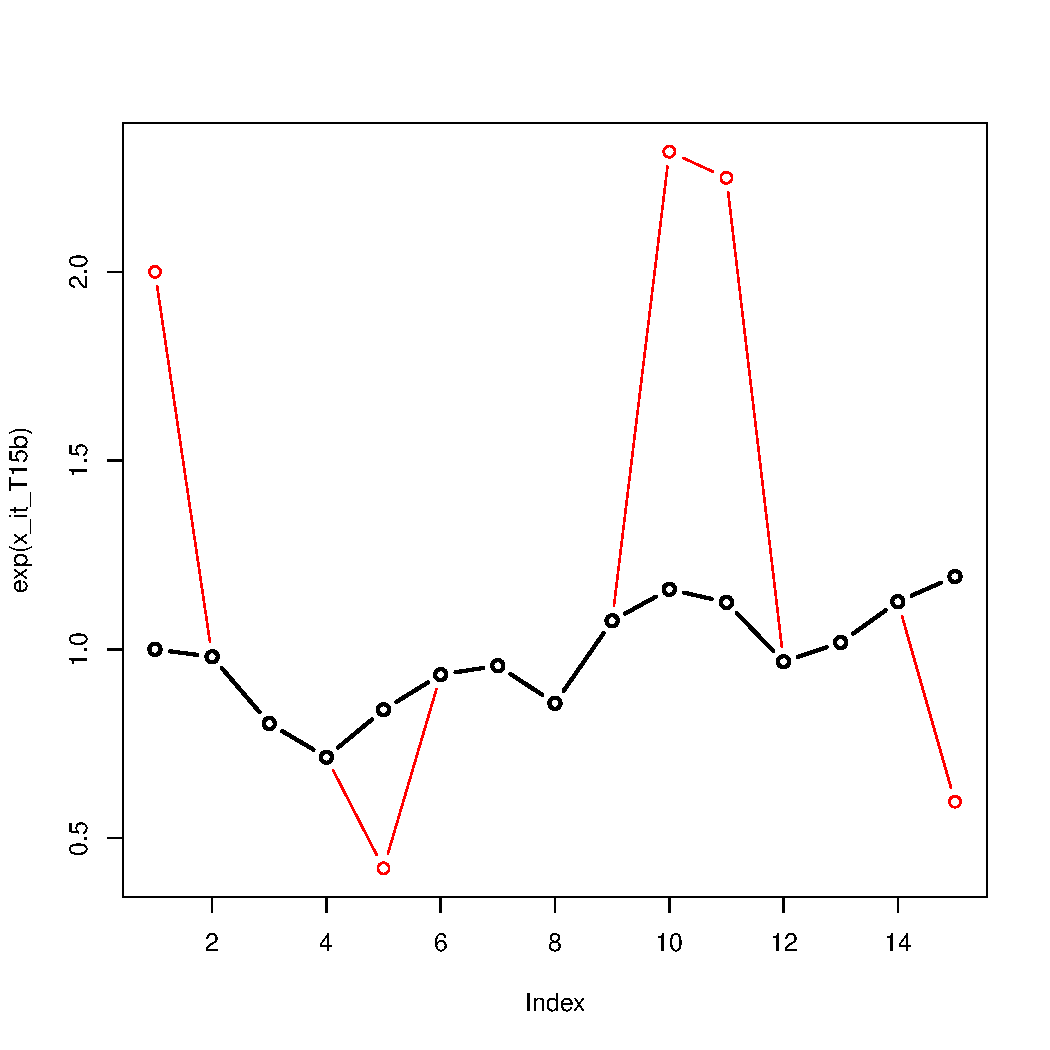
\includegraphics[scale=0.5]{plot_time_effects}
\centering
\end{figure}

\begin{itemize}
\item Check this trend with Marta as the word document and pictured trend are different.
\end{itemize}

In addition to the observed counts at each point we have the expected number of cases for each regions based on true hospital admissions records for each CCG and shape files corresponding to the regions in question.

\subsection{Cleaning and wrangling}

Of the 211 regions one one had no neighbours, the Isle of Wight, so this region was removed to simplify calculations. An adjacency matrix calculated from the shape data. We had no data for wales so it was removed from the shapedata.

\begin{figure}
\centering
\subfloat[Adjacency]{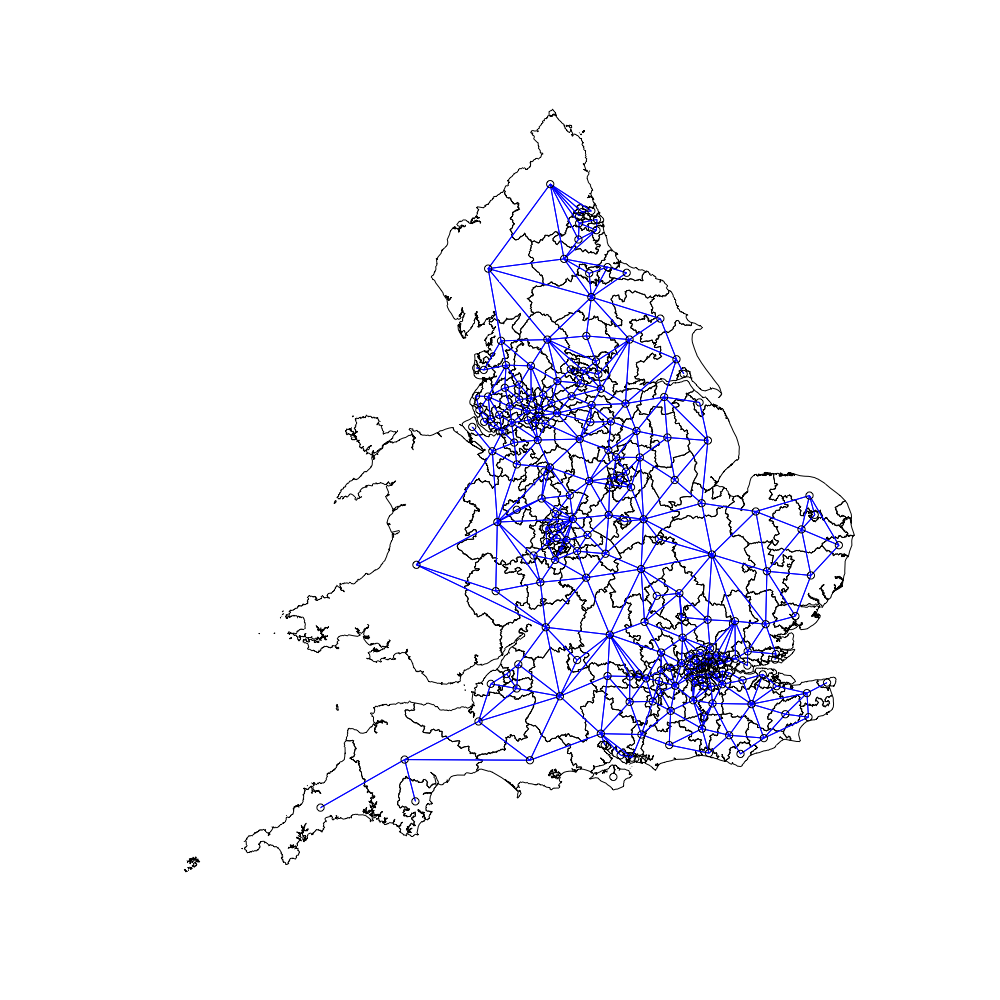
\includegraphics[width=0.5\textwidth]{adjacency}}
\subfloat[Expected]{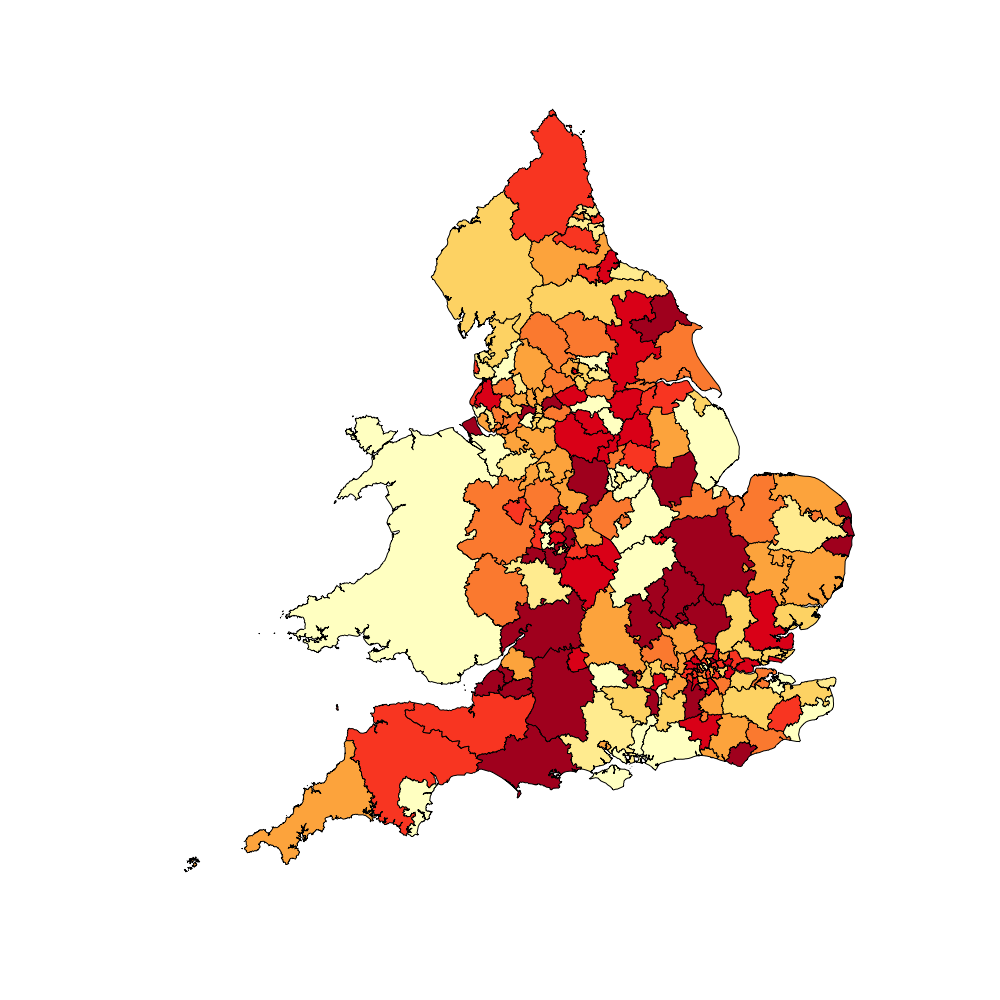
\includegraphics[width=0.5\textwidth]{expected}}
\caption{Mapped data}
\end{figure}

\begin{itemize}
\item Remove wales from the above pictures
\item What to include here?
\end{itemize}


\section{Individual trend model}

The first Bayesian model we wil consider is similar to that which is formed in Someone et al. In this setting we construct two alternate hypothesis for each region, one where the counts at the region are broadly in keeping with some ``global'' temporal trend (subject to localised spatial deviations captured with a conditionally autoregressive prior), and in the other the region has its own individual temporal trend. Then by some method of classification we sort the regions into those deemed most likely to follow the global model and those exhibiting behaviour more typical of the second model - and label these regions ``unusual''.

\subsection{Baystdetect and the cut function}

In the original paper \cite{baystdetect} the use of the cut function in the \emph{BUGS} language is employed to fit the two models to the data seperately and then the model selection is undertaken afterward. This method, which prevents the flow of information between the two models is defended in (Nicky Best presentation here) but has been met with some level of skepticism in the community, for example in Andrew Gelmans posts to the Stan mailing list here (insert link), as the analysis is not ``truly Bayesian''. Nethertheless, we examine this paradigm and compare it to fully Bayesian methods. 

\begin{itemize}
\item Include discussion of model averaging vs larger model
\item Cite Gelman et al 2013
\end{itemize}

\subsubsection{Model specification}

We denote the counts at region $i$ at time $t$ by $Y_{i,t}$ and model them by a Poisson process

\begin{equation}
Y_{i,t} \sim \operatorname{Poisson}(E_{i,t} \cdot \mu_{i,t})
\end{equation}

where $E_{it}$ is the expected count based on population numbers, demographics etc and $\mu_{i,t}$ is the rate parameter by which we impute the two models behaviours. This rate variable we parameterize additively on the log scale for both models as follows

\begin{equation}
\log{(\mu_{i,t})} = \begin{cases}
\ \lambda_{i} + \gamma_{t} \  (+ \  \alpha_0) & \textrm{Model 1 for all } i, t \\
\ u_{i} + \xi_{i,t} & \textrm{Model 2 for all } i, t
\end{cases}
\end{equation} 

Here we see that for Model 1 we assume space-time seperability in the rate paramater with the components given the following priors

\begin{align}
\alpha_0 &\sim \operatorname{Flat}(\mathbb{R}) \\
v_{1:N} &\sim \operatorname{CAR}(W, \sigma_v) \\
\lambda_{1:N} &\sim \operatorname{Normal}(v, \sigma_\lambda) \\
\gamma_{1:T} &\sim \operatorname{RW}(1)
\end{align}

We see here the BYM prior on the spatial component, imposing a smoothing constraint, and a one-dimensional random walk prior on the temporal component. 

The variance hyperparameters are given (insert prior here) as recomended in (possibly Gelman 2006). \\

For the second model we drop the assumption of space-time seperability and each region gets its own temporal trend as follows

\begin{equation}
i \in 1,\ldots,N \
\begin{cases}
\ u_i \sim \operatorname{Normal}(0, 1000) \\
\ \xi_{i, 1:T} \sim \operatorname{RW}(1) 
\end{cases}
\end{equation}

\subsubsection{Implementation}

The two models were fit to the data using Hamiltonian Monte-Carlo in the \emph{Stan} package -- both for over 2000 samples over 4 chains after a ``warm-up'' period of 1000 samples. Gelman-Rubin statistics for all parameters were under 1.05 (find exact figure) indicating that the had chains converged. Additionally a visual inspection of the trace plots for some select parameters did not indicate any worrying pathalogical behaviour.

These two fits took under 5 minutes each to run after a short compilation which is a huge speed increase over typical \emph{BUGS} implementation.

\subsubsection{Classification and accuracy}

First looking at the general trend model we see that it has accurately identified the global temporal trend. 

\begin{figure}
\centering
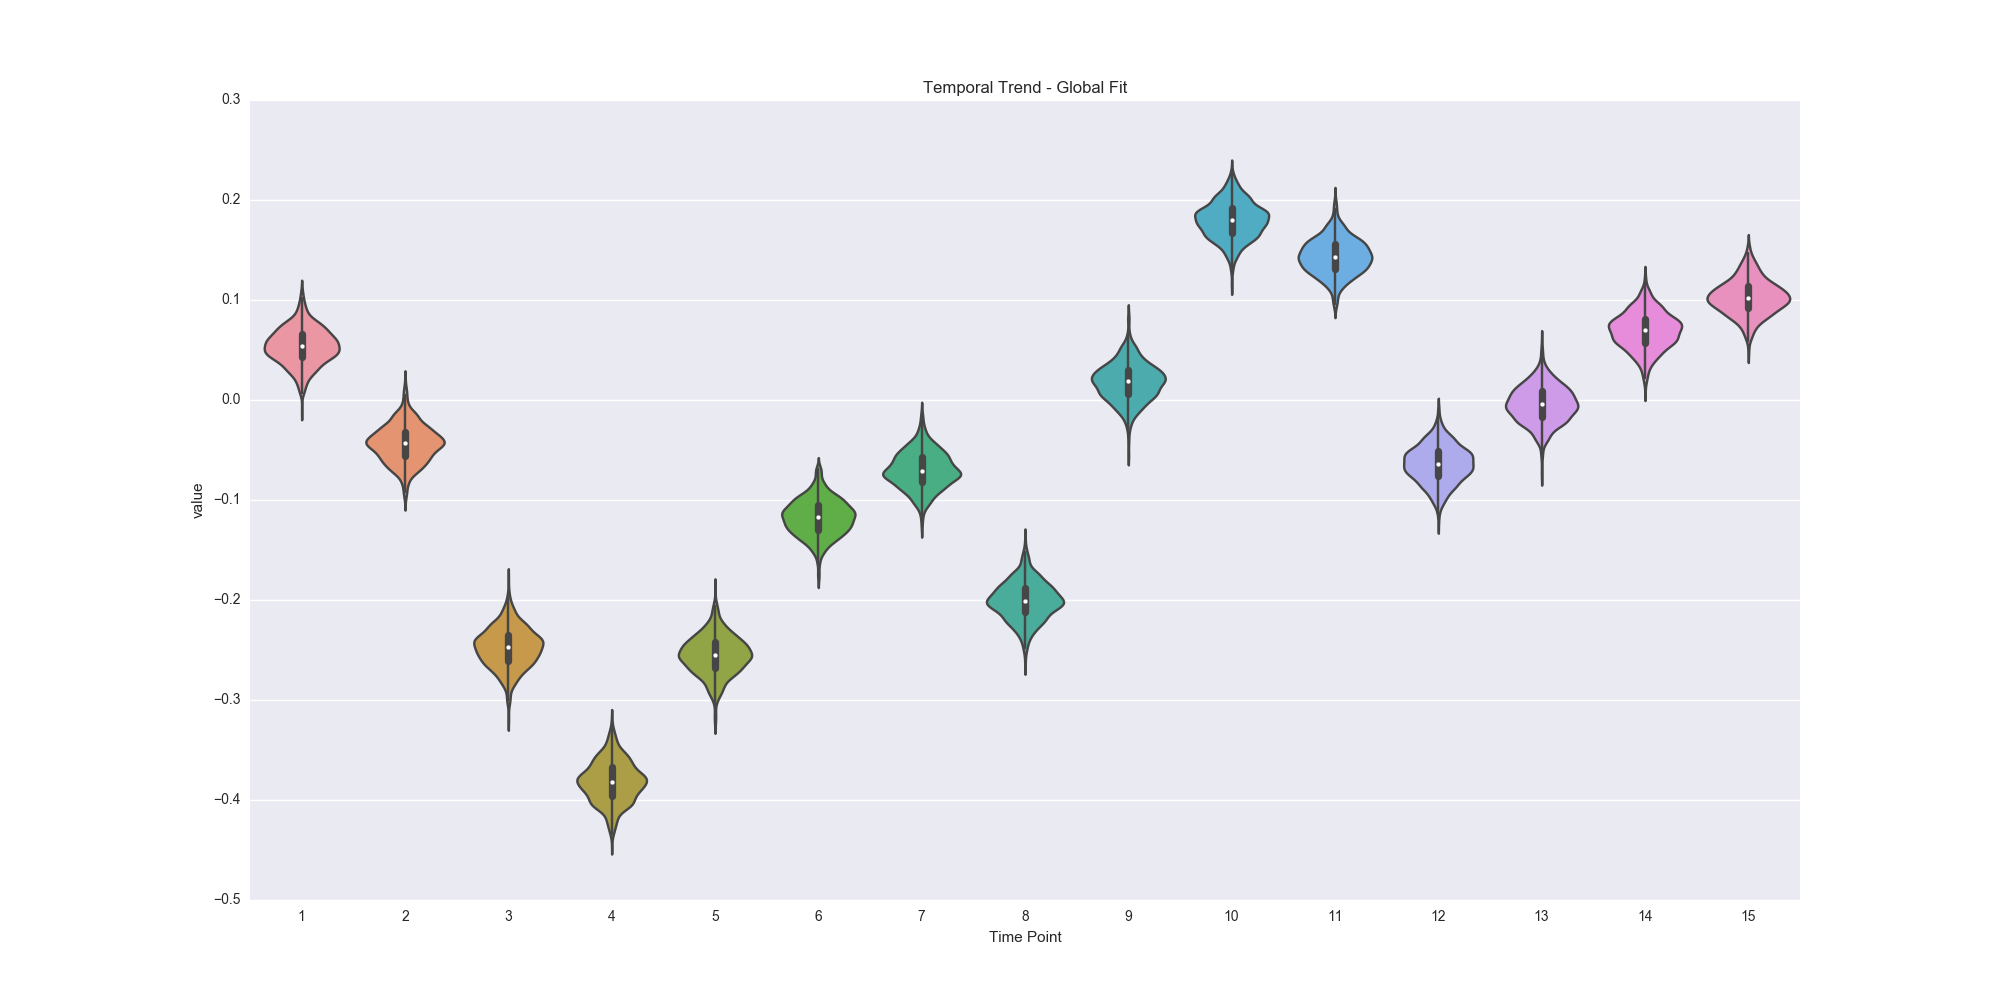
\includegraphics[width=\textwidth]{global_temporal}
\end{figure}

\subsection{Fully Bayesian model}


\section{Excess variability model}

The second Bayesian model we will look at also attempts to classify the regions, into typical and atypical sets, using a mixture model. Here our abnormal regions, rather than coming from an individual temporal trend, simply have excess inseperable spatio-temporal variance. Some potential advantages of such a model compared to Baystdetect are immediately clear:
\begin{itemize}
\item It's relative simplicity allows for easier computation
\item It is not immediately clear that an abnormal temporal trend is symptomatic of an endemic problem --- variance is a more straightforwardly interpretable parameter
\item Identification issues
\end{itemize}

\subsection{Model specification}

The model is similar to that of \cite{stability}, but with a mixture component that's hierachical at the regional level. Like before we model the counts as a Poisson process, $Y_{i,t} \sim \operatorname{Poisson}(E_{i,t} \cdot \mu_{i,t})$, with a rate parameter defined additively on the log-scale

\begin{equation}
\log(\mu_{i,t}) = \lambda_i + \gamma_t + \psi_{i,t}
\end{equation}

where, as before,
\begin{align}
v_{1:N} &\sim \operatorname{CAR}(W, \sigma_v^2) \\
\lambda_{1:N} &\sim \operatorname{Normal}(v, \sigma_\lambda^2) \\
\gamma_{1:T} &\sim \operatorname{RW}(1).
\end{align}

We see the new component $\psi$ captures a level of space-time inseperability to the counts. At every point $(i, t)$ each component is modeled as coming from a mixture of two normal distributions, with the mixture component at the regional level,
\begin{equation}
\psi_{i,t} \sim z_i \cdot \operatorname{Normal}(0, \tau_1^2) + (1 - z_i) \cdot \operatorname{Normal}(0, \tau_2^2)
\end{equation} 

where
\begin{equation}
  z_i \sim \operatorname{Bernoulli}(q_i)
\end{equation}

<<<<<<< HEAD
and the $q_i$ are given Uniform priors on (0, 1). Here we are marginilizing out the $z_i$ and instead performing inference on the $q_i$ which confers the advantages set out under the computational considerations section. The variance parameters are given half-normal priors, one a vague prior (representing the abnormal regions) and the other an informative prior which restricts the inseperable variance of the `normal' regions to be very limited. Identification issues and the label switching problem are avoided by defining the larger of the variances addivitely in terms of the smaller:
=======
and $q$ is given a Uniform prior on (0, 1). The variance parameters are given half-normal priors, one a vague prior (representing the abnormal regions) and the other an informative prior which restricts the inseperable variance of the `normal' regions to be very limited. Identification issues and the label switching problem are avoided by defining the larger of the variances addivitely in terms of the smaller:
>>>>>>> origin/master
\begin{align}
  \tau_1 &\sim \operatorname{Normal}(0, 0.01) \cdot I(0, \infty) \\
  k &\sim \operatorname{Normal}(0, 100) \cdot I(0, \infty)
\end{align}
\begin{equation}
 \tau_2 = \tau_2 + k
\end{equation}

Here $I$ is the indicator function.

\subsection{Classification and accuracy}

<<<<<<< HEAD
This model was fit using HMC in \emph{Stan} 

=======
\subsection{Fully Bayesian model}
>>>>>>> origin/master

\section{Computational considerations}

\subsection{Basic Sampling methods}

\begin{itemize}

\item Mainly using stan for the model

\item Also used BUGS for mixing and speed comparison

\item Discuss pymc3 too and compare with stan's parameter tuning/ initilization with ADVI

\end{itemize}

\subsubsection{Gibbs sampling}

\subsubsection{Metropolis}

\subsection{Hamiltonian Monte-Carlo}

The previous methods, while possessing the desired asymptotic properties, can---and do---take a long time to converge to the target distribution (infinity is a long time!). The aim of \emph{Hamiltonian Monte-Carlo} is to reduce the correlations between successive samples and so dramatically increase the effective sample size with minimal computational overhead. It does this by introducing an auxilliary variable and exploiting the interplay between this and the variables of the posterioir distribution within the framework of Hamiltonian mechanics.

\subsubsection{Background}

We write $q$ for the variables of the posterior distribution and introduce a new variable $p$ which we will call the \emph{momentum} of the system. Drawing from statistical mechanics, we know that for a given energy function of a system $E(\theta)$ we have the canonical ensemble
\begin{equation}
  p(\theta) = \frac{1}{Z} e^{-E(\theta)}.
\end{equation}

So defining a Hamiltonian of our system where the ``kiniteic energy'' is dependent on our momentum and the potential energy is dependent only on the posterioir:
\begin{equation}
  H(p, q) = \underbrace{T(p|q)}_{\text{Kinetic energy}} + \underbrace{V(q)}_{\text{Potential energy}}
\end{equation} 

looking at the canonical ensemble of the join distribution
\begin{align}
  \pi(p, q) &\;{\propto} \; e^{-H(p, q)} \\
          &= e^{-[T(p|q) + V(q)]} \\
          &= e^{-T(p|q)} \cdot e^{-V(q)} \\
          &\;{\propto} \; \pi(p|q) \cdot \pi(q) 
\end{align}

we see that the posterior and distribution of the momentum are seperable and so independent. This means that if we can sample from $\pi(p, q)$ then our choice of distirbution for the momentum will not effect the calculation of any expectations based on the samples of $q$. \\

Note that here we need a definition of potential energy which will give us back the posterior. Clearly the following satisfies this requirement
\begin{equation}
  V(q) = - \log \pi(q)
\end{equation}

So draws from $\pi(p, q)$ will allow us to make inferences on the $q$, but what advantages does the introduction of this auxilliary variable confer? Well, continuing with our intuition regarding a physical Hamiltonian system, we know that $p$ and $q$ are related by Hamilton's equations
\begin{align}
\frac{dq}{dt} &= \frac{\partial H}{\partial p} = \frac{\partial T}{\partial p} \\
\frac{dp}{dt} &= - \frac{\partial H}{\partial q} = - \frac{\partial T}{\partial q} - \frac{\partial V}{\partial q}
\end{align}

\begin{itemize}
  \item Finish off this bit more gracefully
\end{itemize}

\subsubsection{The Method}
<<<<<<< HEAD
=======

Hamiltonian monte-carlo works, not by applying a transition over $q$, but by giving our starting point ``a kick'' in the form of a random momentum and sampling along the level set of constant energy (defined by the Hamiltonian) using Hamilton's equations to evolve the joint system. Then---after some number of steps---we stop, sample a new momentum, and explore the new phase space that this defines. \\

The questions now are obvious:
>>>>>>> origin/master

Hamiltonian monte-carlo works, not by applying a transition over $q$, but by giving our starting point ``a kick'' in the form of a random momentum and sampling along the level set of constant energy (defined by the Hamiltonian) using Hamilton's equations to evolve the joint system. Then---after some number of steps---we stop, sample a new momentum, and explore the new phase space that this defines. \\

The questions now are obvious:

\begin{itemize}
\item \emph{How} do we evolve the joint system in accordance with Hamilton's equations?
\item Do we need to work out all of the partial deriavtives $\partial V/\partial q_i$ by hand? 
\item For how long should we explore each level set before sampling a new momentum?
\item What proposal density should we use for the momentum?
\item Why does this method lead to samples with less autocorrelation?
\end{itemize}

Other things to talk about:
\begin{itemize}
\item \emph{How} do we evolve the joint system in accordance with Hamilton's equations?
\item Do we need to work out all of the partial deriavtives $\partial V/\partial q_i$ by hand? 
\item For how long should we explore each level set before sampling a new momentum?
\item What proposal density should we use for the momentum?
\item Why does this method lead to samples with less autocorrelation?
\end{itemize}

Other things to talk about:
\begin{itemize}

\item Rotational invariance

\item Include some diagrams from Michael Betancourt's papers
<<<<<<< HEAD
=======

\end{itemize}

\subsubsection{Auto differentiation}

\subsubsection{Symplectic Integration}
>>>>>>> origin/master

\begin{itemize}
\item Leap-frog integration
\item Metropolis correction
\end{itemize}

<<<<<<< HEAD
\subsubsection{Auto differentiation}

\subsubsection{Symplectic Integration}

\begin{itemize}
\item Leap-frog integration
\item Metropolis correction
\end{itemize}

\subsubsection{Integration time}

\begin{itemize}
\item Naive implementations will not preserve detailed balance
\item Short-time will give large autocorrelations
\item Long-time will face diminishing returns
\item Integration time obviously linear in time, so compare to linear
\item Exhuastive monte-carlo
\item \emph{Identifying the Optimal Integration Time in Hamiltonian Monte-Carlo} (Betancourt 2016)
\end{itemize}

=======
\subsubsection{Integration time}

\begin{itemize}
\item Naive implementations will not preserve detailed balance
\item Short-time will give large autocorrelations
\item Long-time will face diminishing returns
\item Integration time obviously linear in time, so compare to linear
\item Exhuastive monte-carlo
\item \emph{Identifying the Optimal Integration Time in Hamiltonian Monte-Carlo} (Betancourt 2016)
\end{itemize}

>>>>>>> origin/master
\subsection{Autodiff/black-box variational inference?}

\subsection{Reparameterization of the models}

Removing conditional dependencies e.g.

\begin{align*}
\lambda \sim N(v, \sigma^2_\lambda) = N(0, 1) \cdot \sigma_\lambda^2 + v
\end{align*}

\subsection{Marginilizing over the mixture component}

As \emph{Stan} used Hamiltonian Monte-Carlo, which is a gradient based sampler, we can't directly specify a discrete prior as used in mixture models. Instead we can ``marginalize out'' the mixture component to obtain a purely continuous distribution. This also has significan computational benefits (expand on this). \\

Take for example a mixture of two Normal distributions
\begin{equation}
  k \cdot \operatorname{Normal(\mu_1, \sigma_1^2)} + (1 - k) \cdot \operatorname{Normal(\mu_2, \sigma_2^2)}
\end{equation} 
\begin{equation}
  k \sim \operatorname{Bernoulli(\lambda)}.
\end{equation}

In Monte-Carlo we simply need to be able to calculate the posterior at a specific point. Most software, including \emph{Stan}, rather than multiply the posterior by a chain of conditional probability density functions works on the $\log$ scale where to calculate the log posterior we simply need to increment the log posterioir by the log conditional of the hierachical components. So for our mixture of Normals we need to implement the following
\begin{align}
  \text{log\_posterior} &= \text{log\_posterior} + \log(\lambda \cdot \operatorname{Normal\_pdf}(x | \mu_1, \sigma_1^2)  \nonumber \\
                   & \ \ + (1 - \lambda) \cdot \operatorname{Normal\_pdf}(x | \mu_2, \sigma_2^2))
\end{align}

which we can see is continuous. The way we can specifically implement this in \emph{Stan} is by using the following manipulation

\begin{align}
\log(p_X(x | \lambda, \mu_i, \sigma^2_i)) &= \log(\lambda \cdot \operatorname{Normal\_pdf}(x | \mu_1, \sigma_1^2)  \nonumber \\
& \ \ \ \ \ \ \ + (1 - \lambda) \cdot \text{Normal\_pdf}(x | \mu_2, \sigma_2^2)) \\
&= \log(\exp(\log(\lambda \cdot \operatorname{Normal\_pdf}(x | \mu_1, \sigma_1^2)))  \nonumber \\
& \ \ \ \ \ \ \ + \exp(\log((1 - \lambda) \cdot \operatorname{Normal\_pdf}(x | \mu_2, \sigma_2^2)))) \\
&= \operatorname{log\_sum\_exp}(\log(\lambda) + \log\operatorname{Normal\_pdf}(x | \mu_1, \sigma_1^2),  \nonumber \\
& \ \ \ \ \ \ \ \log(1 - \lambda) + \log\operatorname{Normal\_pdf}(x | \mu_2, \sigma_2^2))
\end{align} 

For more on this see page 185 of \cite{stan}.

\begin{itemize}

\item Cite Stan manual

\item Rao-Blackwellization? 

\end{itemize}

\subsection{Timing data?}

<<<<<<< HEAD
\bibliographystyle{apalike}
\bibliography{project}{}
=======
\bibliography{project}{}
\bibliographystyle{plain}
>>>>>>> origin/master

\end{document}
